    \documentclass[a4paper,10pt,twocolumn,fleqn]{article}
    \usepackage{graphicx,url}
    \usepackage[brazil]{babel}   
    \usepackage[utf8]{inputenc} 
    \usepackage[T1]{fontenc} 
    \usepackage{mathtools}
    \usepackage{amsmath}
    \usepackage{amssymb}
    \usepackage{fontawesome}
    \usepackage{booktabs,multirow}
    \usepackage{adjustbox}
    \usepackage{subcaption}
    \usepackage{graphicx}
    \usepackage{ragged2e} 
    \captionsetup{compatibility=false}
    \usepackage{pgfplots}
    \usetikzlibrary{positioning, backgrounds}

    \usepackage{makecell}
    \sloppy
    %\hyphenpenalty=10000
    %\exhyphenpenalty=10000
    \usepackage{mathptmx} %times new roman
    \usepackage[labelsep=endash]{caption}
    \pgfplotsset{compat=1.15} 
    
    %\parindent 5mm
    %\parskip   5mm
    \setlength{\parindent}{5mm} %recuo de texto para cada paragráfo
    \usepackage{indentfirst} %identar 1 paragráfo
 
    %contar referências como capítulo
    \usepackage{etoolbox}
    \patchcmd{\thebibliography}{*}{}{}{}

    %setar margens do documentos
    \usepackage{geometry}
    \geometry{
        a4paper,
        left=20mm,
        top=20mm,
        right=20mm,
        bottom=25mm
    }
    %suprimir data do artigo
    \date{\vspace{-5ex}}
    \date{}
  
  
    %tamanho do texto (2 colunas de 8cm + 1cm de espaço)  
    \textwidth         170mm   
    \columnsep         10mm %espaço entre colunas
    
    %ajuste dos títulos
    \usepackage{titlesec}
    \titleformat{\section}
    {\normalfont\Large\bfseries\itshape\filcenter}{\thesection\hspace{1mm}.}{1mm}{}
    \titleformat{\subsection}
    {\normalfont\Large\bfseries\itshape\filcenter}{\thesubsection\hspace{1mm}.}{1mm}{}
    \titleformat{\subsubsection}
    {\normalfont\Large\bfseries\itshape\filcenter}{\thesubsubsection\hspace{1mm}.}{1mm}{}
    
    \titlespacing\section{0pt}{12pt plus 4pt minus 2pt}{0pt plus 2pt minus 2pt}
    \titlespacing\subsection{0pt}{12pt plus 4pt minus 2pt}{0pt plus 2pt minus 2pt}
    \titlespacing\subsubsection{0pt}{12pt plus 4pt minus 2pt}{0pt plus 2pt minus 2pt}

    % Faz com que a numeração de tabelas seja em formato romano
    \renewcommand{\thetable}{\Roman{table}}

    %header e footer do artigo
    \usepackage{fancyhdr}
    \pagestyle{fancy}
    \fancyhf{}
    \fancyhead[L]{XIV Simpósio de Iniciação Científica, Didática e de Ações Sociais da FEI}
    \renewcommand{\headrulewidth}{1pt}


    \fancyfoot[R]{São Bernardo do Campo -- 2024}
    \renewcommand\footrule{\makebox[\textwidth]{\shadowfill}\\[-2.5\baselineskip]}
    \newcommand\shadowfill{%
        \leavevmode\leaders\hbox{\ooalign{%
                \vrule height 0pt depth 1pt width 1pt}%
        }\hskip\fill\kern0pt%
    }

    %ambiente resumo
    \def\resumo{\normalfont%
        \noindent\Large\bfseries\textit{Resumo}:\normalfont\normalsize%
    }

    %ambiente agradecimentos
    \def\agradecimentos{\normalfont%
        \centering\Large\bfseries\textit{Agradecimentos}\normalfont\normalsize%
    }

    \author{
            \textit{Felipe Estevão Coquito de Mello$^{1}$, Flavio Tonidandel$^{2}$} \\
            \textit{$^{1}$ Engenharia de Mecânica, Centro Universitário FEI} \\
            \textit{$^{2}$ Ciência da Computação, Centro Universitário FEI} \\
            \textit{\{uniefmello, flaviot\}@fei.edu.br}
    }    

    \begin{document} 
        
    %no título não remover o \vspace, é que ele que puxa para o topo da página
    \title{\vspace{-2em}\textbf{Otimização da Estrutura Omnidirecional de um Robô Goleiro}}
   
   
    %não apagar aqui
    \maketitle
    \thispagestyle{fancy}
    
    
    \begin{resumo}
   O estudo tem por objetivo o desenvolvimento de um novo robô omnidirecional para a categoria \textit{Small-Size} da \textit{RoboCup} de futebol de robôs para a equipe RoboFEI, sendo a criação de um robô específico, com a função de ser um goleiro, a fim de melhorar a movimentação horizontal, considerando que atualmente a equipe utiliza o mesmo modelo de robô para todas as funções.
    \end{resumo}
    
    \section{Introdução}
    
    A categoria \textit{Small Size League} (SSL) é uma das ligas mais antigas da \textit{RoboCup}, tendo o foco em solucionar o problema da cooperação e controle de robôs inteligentes em ambientes altamente dinâmicos com um sistema híbrido, centralizado/distribuído. Com tal complexidade, é necessário dominar cada aspecto do robô e busca-se a combinação harmônica de diversas áreas do conhecimento para acompanhar o desafio que é estar nesta Liga.

    Para a utilização de um robô na competição, a liga possui regulamentos fixos em relação às especificações que as equipes devem seguir, sendo uma dessas o tamanho máximo dos robôs em campo. É necessário que os jogadores caibam em um cilindro de 180 mm de diâmetro e 150 mm de altura. Existem regras de limite de quanto o robô pode cobrir a área total da bola, entre outras que delimitam o que é um robô da categoria \cite{rules}. Isso cria uma limitação técnica do que é possível incorporar em um novo modelo para a competição. 

    \section{Robôs Omnidirecionais}
    
    Os robôs com rodas Omnidirecionais, também conhecidas como rodas Suíças ou \textit{Mecanum}, têm em seu princípio a capacidade das rodas fornecerem tração na direção normal do motor e paralela ao chão, enquanto a roda pode deslizar sem atrito na direção do eixo do motor \cite{kinematic}.
    
    Essa movimentação que foge do senso comum é possível graças a implementação dos \textit{o-rings} com os roletes. Os \textit{o-rings}, são pequenos toroides feitos de polímero ou elastômero que ficam dispostos perpendicularmente em relação à roda principal. Este conjunto forma a parte mais importante para os sistemas omnidirecionais de deslocamento, são responsáveis pela movimentação para qualquer direção no plano XY sem que o robô necessite deslocar seus eixos de lugar \cite{kinematic}. Um exemplo deste conjunto são as rodas que a equipe RoboFEI utiliza, Figura \ref{fig:rodaExplodida}.

    \begin{figure}[!htb]
        \centering
        \caption{Vista explodida da roda.}
        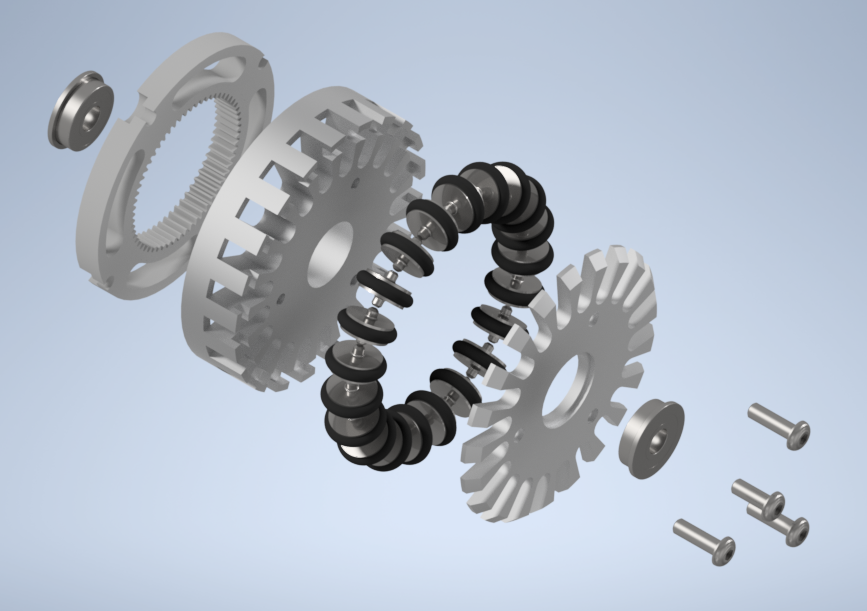
\includegraphics[width=0.7\linewidth]{VistaExplodidaRodaMontada.png}
        \label{fig:rodaExplodida}
    \end{figure}
    
    \subsection{Calculo da Cinemática de Robôs Omnidirecionais Assimétricos}
    
    Os robôs da equipe RoboFEI apresentam atualmente os ângulos $\theta$ e $\phi$ todos simétricos entre si a 33º, o que facilita a construção física e o controle dinâmico do robô. Entretanto, isso prejudica uma otimização do robô para uma função específica. 

    Com isso em mente e levando em conta o trabalho de \cite{rojas2005omnidirectional} onde é abordado a utilização da matriz global de velocidade para robôs omnidirecionais assimétricos, a equipe \cite{Twente} elaborou a partir deste estudo para a categoria SSL um controle no qual é possível retirar a Equação da cinemática direta da matriz de velocidade do robô e a Equação da cinemática inversa,  que representa sua pseudo-inversa, usando como referência a Figura \ref{fig:topview}.

    \begin{figure}[!htb]
        \centering
        \caption{Vista 2D do robô 4 rodas omnidirecionais assimétrico}
        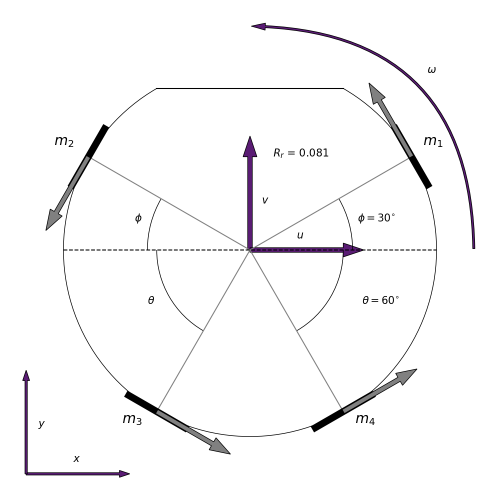
\includegraphics[scale=0.45]{topview.png}
        \label{fig:topview}
    \end{figure}
    
    \begin{table*}
    \centering
    \caption{Tabela de comparação entre os modelos.}\label{tbl:tabelaComparacao}
    \scalebox{1}{%
    \begin{tabular}{ccccccc}
        \toprule
         & \multirow{2}{*}{$V_y max\; [m/s]$} & \multirow{2}{4em}{Numero de ciclos} &
           \multirow{2}{*}{$\Delta_X\; [mm]$} & \multirow{2}{*}{$Maior\; \sigma^2_X\; [mm]$} & \multirow{2}{*}{$Maior\; \sigma^2_X\; [\%]$} &
           \multirow{2}{7em}{Qualidade de movimentação} \\
         & & & & & & \\
        \toprule
        Atual & $1,030$ & $4,50$ & $996,45$ & $36$ & $2,39 \%$ & Alta  \\
        Novo  & $0,751$ & $3,25$ & $990,27$ & $133$ & $13,41 \%$ & Média \\
        \bottomrule
    \end{tabular}
    }
    \end{table*}
    
    \section{Metodologia}

     Analisando as características da equipe RoboFEI, foi desenvolvido um algoritmo para resolver a cinemática direta e inversa do robô estudado. Para validar o funcionamento do código, este foi comparado com a movimentação do robô atual da equipe.
    
     Para a obtenção dos ângulos de otimização, cada combinação de ângulo foi testada individualmente em um percurso estabelecido. Este percurso foi concebido com base na movimentação mais tradicional do robô com função de goleiro durante a partida, onde se desloca majoritariamente na horizontal ($X$), para realizar as defesas da bola em gol, segundo os vídeos que a equipe RoboFEI possui gravados.Após a descoberta do melhor angulo foi feito o projeto mecânico estrutural do novo robô utilizando o software CAD, Autodesk Inventor, tendo em vista as necessidades da equipe. 
    
      Após as usinagens, ocorreram os testes comparativos entre o robô atual e o desenvolvido neste trabalho.
    
    \section{Resultados finais}
    
    Para o estudo dos ângulos, utilizando a matriz inversa, é possível fazer o estudo $\bar{\omega_n}$ que corresponde ao sentido que cada roda deve rotacionar para fornecer a movimentação desejada. Defeinindo os outros valores $Vx$, $Vy$, $\omega$  é possível analisar qual é o comportamento de cada par de ângulo possível de se combinar, em um código em looping. Os resultados das  análises se encontram na Figura \ref{fig:angulo0.1} tendo os melhores resultados numéricos com os ângulos $\alpha$ e $\beta$ sendo iguais a 22º, como o melhor ângulo para o projeto. Com velocidade máxima de 14,08 m/s para. Para garantir mais opções para a modelagem da estrutura caso ocorram restrições geométricas, retiraram-se, além do melhor resultado, os quatro melhores subsequentes: Arranjo 2: $\alpha$ = 22º, $\beta$ = 44º, v$V_y max$ = 14,00 m/s e Arranjo 3: $\alpha$ = 44º, $\beta$ = 22º, $V_y max$ = 14,00 m/s

    \begin{figure}[!htp]
        \centering
        \caption{Representação gráfica da otimização}
        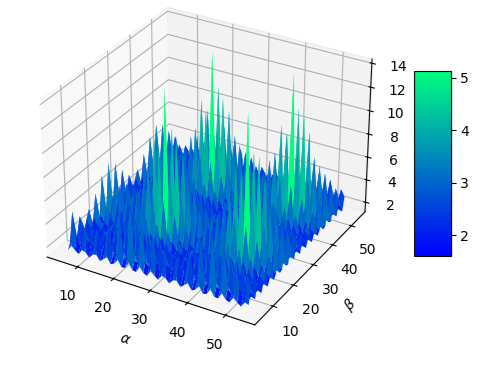
\includegraphics[width=0.8\linewidth]{Figure_0_1_Vx.png}
        \label{fig:angulo0.1}
    \end{figure}

    Após ter construído um robô com os ângulos de $\alpha$ = 22º, $\beta$ = 44º, por conta de ser o único que se abecou aos parâmetros mecânicos. Após a construção, os parâmetro de teste estabelecido foi a maior movimentação que o goleiro pode realizar durante o jogo, sendo este o movimento de ir de uma ponta a outra da sua área de defesa. Com isso, os pontos gerados foram: X 1000 mm, Y -1000 mm e X 1000 mm, Y 1000 mm, sendo assim possível analisar quantos ciclos de defesa cada robô consegue realizar. A linha gerada entre esses dois pontos é uma linha reta com variação apenas no eixo Y Global (eixo X do robô), e ambos os modelos realizarão a mesma trajetória pela mesma quantidade de tempo. Após a finalização do teste de 1 minuto de movimentação para cada robô, foram retirados para análise apenas 30 segundos, a partir da ponta inferior máximo (Posição: -1000 mm).
    
    \section{Conclusões finais}
    
    Após os testes realizados, foi possível notar a diferença da estrutura atual e do proposto pelo projeto. Na Tabela \ref{tbl:tabelaComparacao} é possível notar a tabela de comparação entre os modelos desenvolvidos e o modelo anterior da equipe.
    
    Da mesma forma, observou-se uma grande variança nos resultados na estrutura proposta, chegando a 13,408\% , que corresponde a um trecho 13,3 cm maior do que o estimado. Para trabalhos futuros, seria interessante um estudo mais aprofundado para o controlador deste novo robô, que pode acarretar uma evolução substancial nos resultados deste estudo e trazer melhores frutos para a equipe. Assim como um novo sistema de defesa, aproveitado a maior área frontal gerado pelos novos ângulos.  
    
    %Para criar as referências.
    \bibliographystyle{sicfei}
    
    \bibliography{sicfei}

    \begin{agradecimentos}
    \justify À instituição FEI e à equipe RoboFEI pela realização das medidas e empréstimo do laboratório para testes.
    
    \bigskip % Pula uma linha
    
    $^1$ Aluno de IC do Centro Universitário FEI. Projeto com vigência de 04/23 a 04/24.   
    \end{agradecimentos} 
     
    \end{document}
